% Graphic for TeX using PGF
% Title: /home/araujo/Dropbox/VerbTeX/LivroComputadores/Pictures/memoria.dia
% Creator: Dia v0.97.3
% CreationDate: Sun May 21 11:59:17 2017
% For: araujo
% \usepackage{tikz}
% The following commands are not supported in PSTricks at present
% We define them conditionally, so when they are implemented,
% this pgf file will use them.
\ifx\du\undefined
  \newlength{\du}
\fi
\setlength{\du}{15\unitlength}
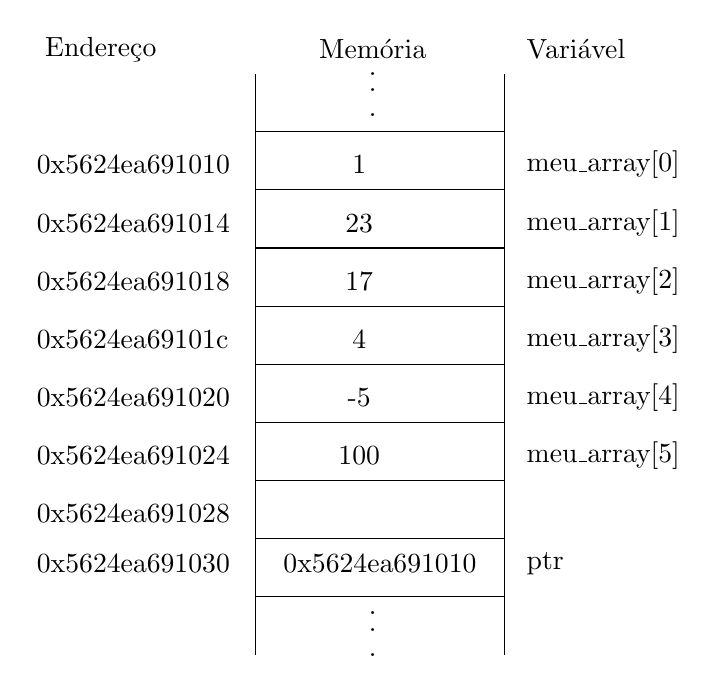
\begin{tikzpicture}
\pgftransformxscale{1.000000}
\pgftransformyscale{-1.000000}
\definecolor{dialinecolor}{rgb}{0.000000, 0.000000, 0.000000}
\pgfsetstrokecolor{dialinecolor}
\definecolor{dialinecolor}{rgb}{1.000000, 1.000000, 1.000000}
\pgfsetfillcolor{dialinecolor}

\draw (31\du,9.4\du)--(31.\du,8\du)--(25\du,8\du)--(25\du,9.4\du);
\node at (27.5\du,8.8\du){1};
\draw (31\du,10.8\du)--(31.\du,9.4\du)--(25\du,9.4\du)--(25\du,10.8\du);
\node at (27.5\du,10.2\du){23};
\draw (31\du,12.2\du)--(31.\du,10.8\du)--(25\du,10.8\du)--(25\du,12.2\du);
\node at (27.5\du,11.6\du){17};
\draw (31\du,13.6\du)--(31.\du,12.2\du)--(25\du,12.2\du)--(25\du,13.6\du);
\node at (27.5\du,13\du){4};
\draw (31\du,15\du)--(31.\du,13.6\du)--(25\du,13.6\du)--(25\du,15\du);
\node at (27.5\du,14.4\du){-5};
\draw (31\du,16.4\du)--(31.\du,15\du)--(25\du,15\du)--(25\du,16.4\du);
\node at (27.5\du,15.8\du){100};
\draw (31\du,17.8\du)--(31.\du,16.4\du)--(25\du,16.4\du)--(25\du,17.8\du);
\node at (28\du,18.4\du){0x5624ea691010};
\draw (31\du,17.8\du)--(31.\du,16.4\du)--(25\du,16.4\du)--(25\du,17.8\du);
%\node at (27.5\du,18.6\du){0110 1100};
\draw (31\du,19.2\du)--(31.\du,17.8\du)--(25\du,17.8\du)--(25\du,19.2\du)--cycle;
\node[anchor=west] at (27.5\du,20.6\du){.};
\node[anchor=west] at (27.5\du,20\du){.};
\node[anchor=west] at (27.5\du,19.6\du){.};

\definecolor{dialinecolor}{rgb}{0.000000, 0.000000, 0.000000}
\pgfsetstrokecolor{dialinecolor}
\draw (25\du,19.2\du)--(25\du,20.6\du);
\draw (31\du,19.2\du)--(31\du,20.6\du);
\draw (25\du,6.6\du)--(25\du,8\du);
\draw (31\du,6.6\du)--(31\du,8\du);
\node[anchor=west] at (27.5\du,7.600000\du){.};
\node[anchor=west] at (27.5\du,7.000000\du){.};
\node[anchor=west] at (27.5\du,6.600000\du){.};
\node[anchor=west] at (19.5\du,8.8\du){0x5624ea691010};
\node[anchor=west] at (19.5\du,10.2\du){0x5624ea691014};
\node[anchor=west] at (19.5\du,11.6\du){0x5624ea691018};
\node[anchor=west] at (19.5\du,13\du){0x5624ea69101c};
\node[anchor=west] at (19.5\du,14.4\du){0x5624ea691020};
\node[anchor=west] at (19.5\du,15.8\du){0x5624ea691024};
\node[anchor=west] at (19.5\du,17.2\du){0x5624ea691028};
\node[anchor=west] at (19.5\du,18.4\du){0x5624ea691030};
\node[anchor=west] at (19.7\du,6.002347\du) {Endere\c{c}o};
\node[anchor=west] at (26.3\du,6.002347\du){Mem\'{o}ria};
\node[anchor=west] at (31.3\du,6.002347\du){Vari\'{a}vel};
\node[anchor=west] at (31.3\du,8.8\du){meu\_array[0]};
\node[anchor=west] at (31.3\du,10.2\du){meu\_array[1]};
\node[anchor=west] at (31.3\du,11.6\du){meu\_array[2]};
\node[anchor=west] at (31.3\du,13\du){meu\_array[3]};
\node[anchor=west] at (31.3\du,14.4\du){meu\_array[4]};
\node[anchor=west] at (31.3\du,15.8\du){meu\_array[5]};
\node[anchor=west] at (31.3\du,18.4\du){ptr};
\end{tikzpicture}
